\section{Additional Details for the Number-Comparison Probe}
\label{app:number-comparison}

This appendix provides additional details for the controlled number-comparison probe introduced in~\cref{sec:reasoning}. The probe measures whether a model assigns higher likelihood to the numerically correct candidate in a pairwise comparison, rather than evaluating unrestricted mathematical generation.

\subsection{Synthetic Task Construction}
\label{app:number-comparison-task}

Each example contains two integers $(a,b)$ and an instruction asking for either the larger or the smaller value. We generate pairs as
\begin{equation}
    (a,b)=(n,n+d),
    \label{eq:app-fixed-gap-pair}
\end{equation}
where $n$ is sampled from one of four magnitude groups and $d$ is a fixed absolute gap. The magnitude groups are
\begin{equation}
\mathcal{G}_1=[10,99],\quad
\mathcal{G}_2=[100,999],\quad
\mathcal{G}_3=[1000,9999],\quad
\mathcal{G}_4=[10000,99999].
\label{eq:app-magnitude-groups}
\end{equation}
We use two gap regimes:
\begin{equation}
\mathrm{SG}=\{1,2,3,4,5\},\qquad
\mathrm{MG}=\{6,7,8,9,10\}.
\label{eq:app-gap-regimes}
\end{equation}
For each magnitude group and exact gap, we sample 32 starting values with a fixed seed. We include both candidate orderings, $(a,b)$ and $(b,a)$, and both query directions, ``larger'' and ``smaller'', so the benchmark is balanced against positional and lexical shortcuts.

\begin{table}[h!]
\centering
\resizebox{\linewidth}{!}{%
\begin{tabular}{lcc}
\toprule
Component & Count & Description \\
\midrule
Magnitude groups & 4 & $\mathcal{G}_1$--$\mathcal{G}_4$ \\
Gap regimes & 2 & SG and MG \\
Exact gaps per regime & 5 & $d\in\{1,\ldots,5\}$ or $d\in\{6,\ldots,10\}$ \\
Starting values per exact gap & 32 & Fixed random seed \\
Candidate orderings & 2 & $(a,b)$ and $(b,a)$ \\
Directions & 2 & larger and smaller \\
Exemplar sets & 3 & Robustness over few-shot examples \\
\midrule
Total per model-shot condition & 15{,}360 & $4\times2\times5\times32\times2\times2\times3$ \\
\bottomrule
\end{tabular}}
\caption{Construction of the synthetic number-comparison benchmark. The design balances magnitude, gap, answer order, and query direction.}
\label{tab:app-comparison-task-breakdown}
\end{table}

\subsection{Likelihood-Based Scoring}
\label{app:number-comparison-scoring}

For a prompt $q$, the valid continuations are the two candidate numbers $c_a$ and $c_b$. We score each candidate using length-normalized log-likelihood:
\begin{equation}
    s(c\mid q)=\frac{1}{|c|}\sum_{t=1}^{|c|}\log p(c_t\mid q,c_{<t}),
    \label{eq:app-candidate-score}
\end{equation}
where $|c|$ is the number of tokens in the candidate continuation. The model prediction is
\begin{equation}
    \hat{c}=\arg\max_{c\in\{c_a,c_b\}} s(c\mid q).
    \label{eq:app-candidate-selection}
\end{equation}
Accuracy is then
\begin{equation}
    \mathrm{Acc}=\frac{1}{M}\sum_{j=1}^{M}\mathbb{I}[\hat{c}_j=c_j^\star],
    \label{eq:app-comparison-accuracy}
\end{equation}
with $M=15{,}360$ examples per model-shot condition. This evaluation avoids sampling variance and measures the model's relative preference between the two numerical candidates.

\subsection{Few-Shot Results}
\label{app:number-comparison-fewshot-results}

\begin{table}[h!]
\centering
\begin{tabular}{ccccc}
\toprule
Shots & $\rho_s$ & Pearson $r$ & $R^2$ & Mean Acc. \\
\midrule
0 & 0.84 & 0.80 & 0.64 & 0.64 \\
1 & 0.83 & 0.80 & 0.64 & 0.63 \\
2 & 0.74 & 0.79 & 0.62 & 0.62 \\
3 & 0.80 & 0.81 & 0.65 & 0.62 \\
4 & 0.82 & 0.85 & 0.72 & 0.62 \\
\bottomrule
\end{tabular}
\caption{Correlation between PCA scaling factor $\beta$ and number-comparison accuracy across shot settings. Correlations are computed across the 14 evaluated base models.}
\label{tab:app-shot-correlation-summary}
\end{table}

\begin{figure}[h!]
\centering
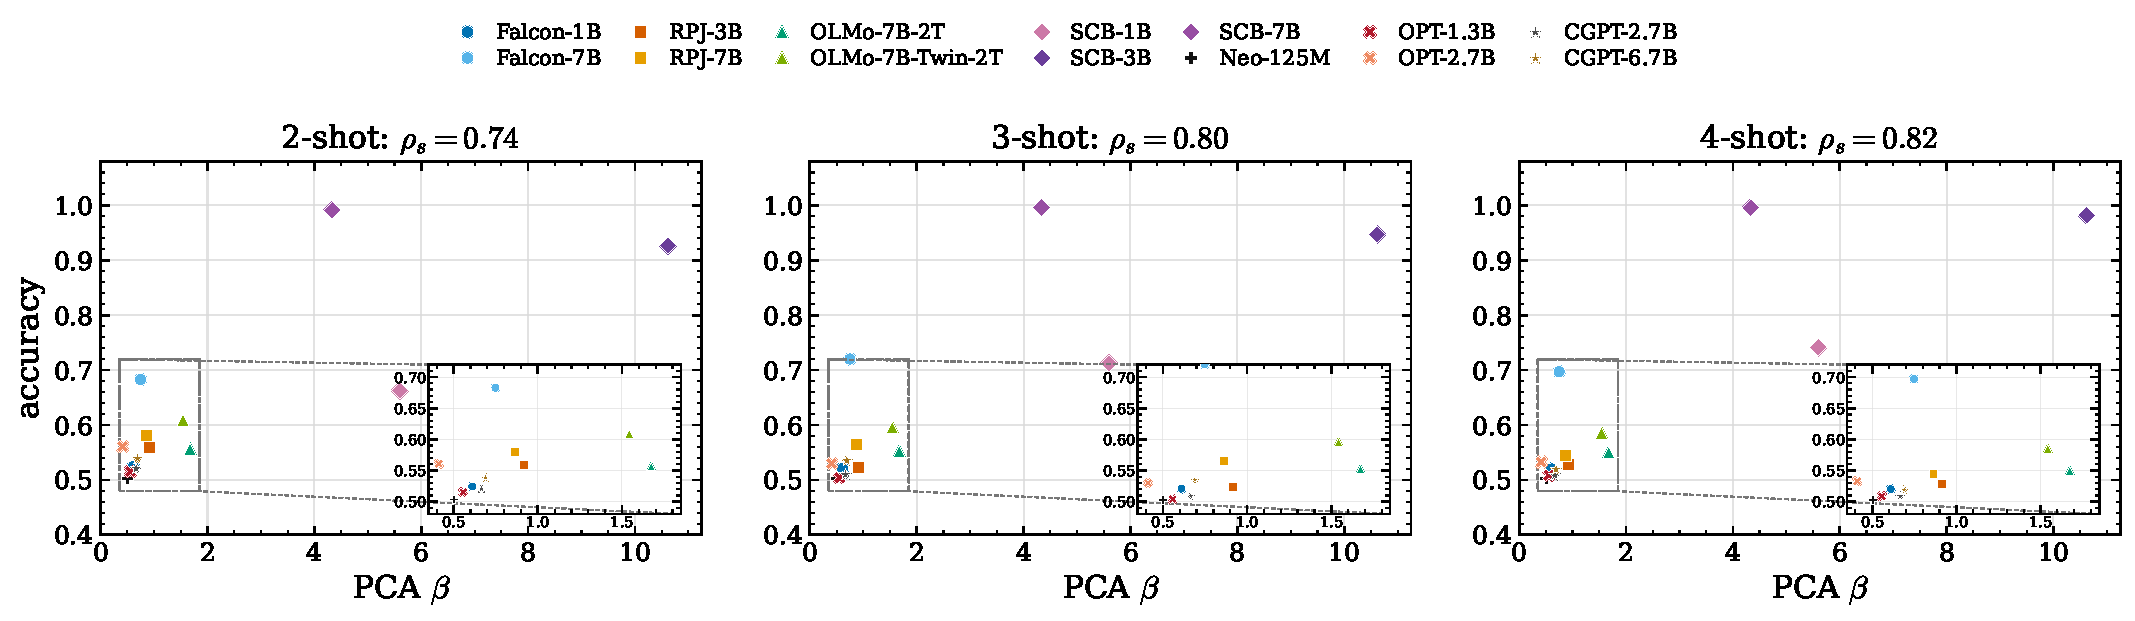
\includegraphics[width=0.9\linewidth]{figs/2-4.pdf}
\caption{Number-comparison accuracy versus PCA scaling factor $\beta$ for 2-, 3-, and 4-shot settings. Each point is one model; the inset zooms into the low-$\beta$ region.}
\label{fig:app-comparison-2-4}
\end{figure}

The positive Spearman correlations in~\cref{tab:app-shot-correlation-summary} show that the $\beta$--accuracy relationship is not specific to the zero-shot prompt. The relationship remains positive from 1-shot through 4-shot prompting, and the 2--4 shot panels in~\cref{fig:app-comparison-2-4} show the same qualitative pattern as the main 0--1 shot figure.

\subsection{Per-Model Shot Accuracy}
\label{app:number-comparison-per-model}

\begin{table}[h!]
\centering
\resizebox{\linewidth}{!}{%
\begin{tabular}{llccccccc}
\toprule
Model & Family & $\beta$ & Type & 0-shot & 1-shot & 2-shot & 3-shot & 4-shot \\
\midrule
Falcon-1B & Falcon & 0.61 & baseline & 0.519 & 0.530 & 0.524 & 0.521 & 0.520 \\
Falcon-7B & Falcon & 0.75 & baseline & 0.633 & 0.647 & 0.683 & 0.720 & 0.697 \\
RPJ-3B & RedPajama & 0.92 & baseline & 0.556 & 0.566 & 0.559 & 0.523 & 0.529 \\
RPJ-7B & RedPajama & 0.86 & baseline & 0.528 & 0.599 & 0.580 & 0.565 & 0.545 \\
OLMo-7B-2T & OLMo & 1.67 & baseline & 0.686 & 0.582 & 0.557 & 0.552 & 0.550 \\
OLMo-7B-Twin-2T & OLMo & 1.54 & baseline & 0.694 & 0.614 & 0.609 & 0.596 & 0.585 \\
SCB-1B & StarCoderBase & 5.60 & baseline & 0.737 & 0.676 & 0.663 & 0.713 & 0.741 \\
SCB-3B & StarCoderBase & 10.62 & baseline & 0.897 & 0.922 & 0.926 & 0.947 & 0.982 \\
SCB-7B & StarCoderBase & 4.33 & baseline & 0.974 & 0.991 & 0.991 & 0.996 & 0.996 \\
CGPT-2.7B & Cerebras-GPT & 0.67 & candidate & 0.568 & 0.537 & 0.521 & 0.509 & 0.508 \\
CGPT-6.7B & Cerebras-GPT & 0.69 & candidate & 0.599 & 0.542 & 0.539 & 0.535 & 0.519 \\
Neo-125M & GPT-Neo & 0.50 & candidate & 0.500 & 0.502 & 0.503 & 0.503 & 0.503 \\
OPT-1.3B & OPT & 0.56 & candidate & 0.541 & 0.554 & 0.515 & 0.504 & 0.508 \\
OPT-2.7B & OPT & 0.41 & candidate & 0.534 & 0.566 & 0.561 & 0.530 & 0.533 \\
\bottomrule
\end{tabular}}
\caption{Per-model number-comparison accuracy across shot settings. Candidate models are included only in the behavioral comparison because their exact pretraining corpora are not matched in the corpus-frequency analysis.}
\label{tab:app-per-model-shot-accuracy}
\end{table}

\subsection{Interpretation of the Behavioral Probe}
\label{app:number-comparison-interpretation}

The number-comparison probe should be interpreted as a controlled preference test. Since both candidate answers are scored directly, the result is not affected by stochastic decoding or by whether the model chooses to emit explanatory text. However, it is still not a complete measure of mathematical reasoning: it tests pairwise numerical discrimination under a fixed prompt format. The consistent positive relationship between $\beta$ and accuracy in~\cref{tab:app-shot-correlation-summary,tab:app-per-model-shot-accuracy} supports the main claim that less compressed number-line geometry is associated with better numerical comparison behavior.
